\chapter{Experiments\label{chap:experiments}}

We implemented  all variants and refinements of \algname{} described in Section~3 in C++. The implementation and data will be made available in open source and are available for reviewing purposes in the supplement. Our implementations of MSU3 and OLL were inspired by their implementations in Open-WBO~\autocite{DBLP:conf/sat/MartinsML14},
the other variants were implemented from scratch.
We used CaDiCaL~\autocite{BiereFazekasFleuryHeisinger-SAT-Competition-2020-solvers} as the internal SAT solver.
We also reimplemented the competing approaches considered (see \cref{sec:competing}),
since no reference implementations were available.
We evaluate the relative runtime performance of the \algname{} variants against two competing approaches, as well
as the impact of the specific refinements (recall Section~3.3, employed as applicable by default, with heuristic core minimization) to \algname{} on its runtime performance.
As a parametric detail, in its default \msh{} is configured to switch between \msu{} and \satunsat{} once 70\% of the literals in $\Obj_\inc$ have been added to $\tot(\Act)$.
All experiments were run on 2.60-GHz Intel Xeon E5-2670 machines with 64-GB RAM in RHEL under a 1.5-hour per-instance
time  and 16-GB memory limit. 

\section{Benchmarks\label{sec:benchmarks}}

\subsection{Learning Interpretable Decision Rules\label{sec:lidr}}

Recently, a variety of SAT and MaxSAT-based approaches have been developed for
learning interpretable classifiers from data~\autocite{DBLP:conf/ijcai/Ignatiev0NS21,DBLP:conf/cp/MaliotovM18,DBLP:conf/ijcai/NarodytskaIPM18,DBLP:conf/ijcai/Hu0HH20,DBLP:journals/corr/abs-2010-09919,DBLP:conf/cp/YuISB20,DBLP:conf/cade/IgnatievPNM18}. The two objectives
of minimizing size (the smaller, the more interpretable) and classification error
(when there is no perfect classifier, as typical for real-world data) are conflicting,
hence giving naturally rise to bi-objective optimization problems.
Here we consider learning of interpretable decision rules as a representative benchmark domain
from this line of work, building on the encoding presented in~\textcite{DBLP:conf/cp/MaliotovM18}.
In short, here  a decision rule is a binary classifier in the form of a CNF formula over boolean features.
In~\textcite{DBLP:conf/cp/MaliotovM18} a linear combination of the
two objectives, using a parameter $\lambda\geq 0$,  was proposed in order to directly apply a MaxSAT solver
to find decision rules under a pre-fixed value for $\lambda$.
While this allows for finding a pareto-optimal decision rule under a specific value of $\lambda$,
MaxSAT solving multiple times under different choices of $\lambda$ does not  guarantee finding
a representative pareto-optimal  decision rule for each pareto point~\autocite{survey}.
In contrast, here we address directly the
problem of computing all pareto-optimal solutions wrt the two objectives.
For a gives set of $\nsamp$ data samples over $\nfeat$ features
the encoding uses two sets of variables: $\selector_l^j$ for $l=1,\dots,\nclauses$, $j=1,\dots,\nfeat$ and $\noise_i$ for $i=1,\dots,\nsamp$
for a specific number  $\nclauses$ of clauses in the  decision rules to be learned,
with the interpretation that $\selector_l^j=1$ iff
the $j$th feature is included in the $l$th clause of the decision rule, and $\noise_i=1$ if the $i$th
data sample is misclassified.

We represent the sample with index $i$ with a boolean class $y_i$ and the boolean features $x_i^j$ where $j=1,\dots,\nfeat$.
With this, the encoding is $\lnot \noise_i \rightarrow (y_i \leftrightarrow \bigwedge_{l=1}^\nclauses \bigvee_{j=1}^\nfeat (x_i^j \land \selector_l^j))$.
We use this encoding, literals $\selector_l^j$ as $\Obj_\inc$ and literals $\noise_i$ as $\Obj_\dec$.
This corresponds to finding pareto-optimal solutions wrt the size of the decision rule as the total number of literals and its classification error.
(In preliminary experiments we observed that using the classification error as the increasing objective leads to worse performance.)
Since decision rules in CNF contain many symmetric solutions obtained by changing the order of clauses, we
add additional clauses to the encoding to break these symmetries by enforcing a lexicographic ordering on the bit-strings
representing the clauses; see \cref{sup:symbr} (in the supplement) for details.


As the basis of benchmark instances, we used
24 standard UCI~\autocite{UciMlr} and Kaggle datasets % ({\small\url{https://www.kaggle.com}}) benchmark datasets, including ones
used in~\textcite{DBLP:conf/cp/MaliotovM18}; see \cref{sup:datasets} for details.
We randomly and independently sampled subsets of $\nsamp\in\{50,100,1000,5000,10000\}$ data samples from the datasets, four of each size (when applicable), resulting in a
total of 372 datasets. %, and discretized the data as in~\cite{DBLP:conf/cp/MaliotovM18}:
%categorical features are one-hot encoded, continuous features discretized by comparing to a collection of thresholds.
All experiments on these datasets where run with the encoding from~\textcite{DBLP:conf/cp/MaliotovM18} configured to learn CNF decision rules consisting of two clauses.

When enumerating multiple solutions corresponding to the same pareto point, the blocking clauses for \algname{} (as
well as the $P$-minimal approach compared to in the experiments) can be strengthened
to find solutions mapping to distinct rules: blocking over the variables $s_l^j$ is sufficient and blocks multiple
symmetric solutions that only differ in the assignment to auxiliary variables.
%Since we want to find solutions corresponding to distinct rules, blocking a solution $\tau$ with $\{ \lnot s_l^j \mid l=1,\dots,\nclauses,\,j=1,\dots,\nfeat,\,\tau(s_l^j)=1 \} \c\up \{ s_l^j \mid l=1,\dots,\nclauses,\,j=1,\dots,\nfeat,\,\tau(s_l^j)=0 \}$ is sufficient and blocks multiple symmetric solutions that only differ in the assignment to auxiliary variables.
Further, making use of the algorithm-specific fact that \algname{} is guaranteed to enumerate pareto-optimal solutions in order of increasing size,
for \algname{} it is sufficient to block a solution over all $s_l^j$ that are assigned to false.

\subsection{Bi-Objective Set Covering}

In the set covering problem over sets $\sets$, a subset $\cover$ of the elements $\{1,\dots,\nelems\}$ needs to be
chosen such that (i)~$\cover$ covers all sets in $\sets$, i.e., $\cover\cap S\neq\emptyset,\,\forall S\in\sets$, and (ii)~$\cover$ is minimal regarding some objective.
The bi-objective variant assigns each element $\element$ two different cost values $\cost^\element_1$ and $\cost^\element_1$ where the two
different objectives for the cover $\cover$ are to minimize $\sum_{\element\in\cover}\cost^\element_1$ and $\sum_{\element\in\cover}\cost^\element_2$.
When encoding set covering into propositional logic, every set $S\in\sets$ forms one clause in the encoding, i.e., the clauses are $\{l_\element \mid \element\in S\}$
with $l_\element$ being a literal representing if element $\element$ is in $\cover$.
Furthermore, the integer values for the cost associated with element $\element$ can be represented by adding $l_\element$ to the objective set $\cost^\element$ times.
Note that multi-objective set covering was also used originally for evaluating $P$-minimal~\autocite{DBLP:conf/cp/SohBTB17}.

We generated two types of  bi-objective set covering problem instances:
(i)~using a fixed probability $\elemprob$ for an element appearing in a set (SetCovering-EP), and (ii)~using fixed set cardinality $\setcard$,
with elements in a set chosen uniformly at random without replacement (SetCovering-SC).
We generated both types of instances using combinations of the following parameters: number of elements $\nelems\in\{100,150,200\}$,
number of sets $\nsets\in\{20,40,60,80\}$, element probability $\elemprob\in\{0.1,0.2\}$ and set cardinality $\setcard\in\{5,10\}$.
For each combination, we generated five instances, leading to 120 instances of each type.
The integer cost values $\cost$ for the two objectives where chosen uniformly at random from the range $\cost\in[1,100]$.

The blocking clauses used in \algname{} for enumerating all pareto-optimal solutions can be strengthened also for set covering:
due to the fact that \algname{} is guaranteed to enumerate the pareto-optimal solutions
so that one of the objectives will monotonically decrease, it is enough to block in \algname{} the
solution over all $l_e$ that are assigned to true.

\section{Results\label{sec:results}}

\begin{figure}
    \centering
    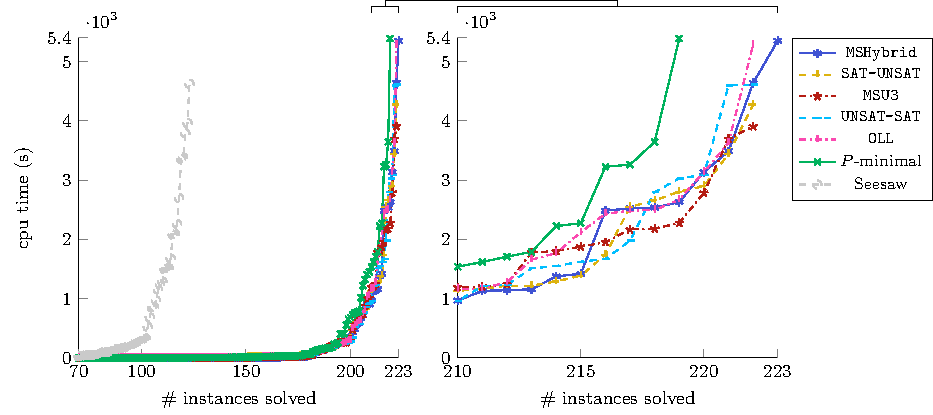
\includegraphics{mlic-cactus-single.pdf}
    \caption{Runtime comparison of  $P$-minimal and variants of \algname{} for LIDR; plot on the right
      is zoomed in on the more interesting part of the left plot.
      %        On the right, a magnified version from 195 solved instances on is shown.
    }\label{fig:mlic-cactus}
\end{figure}

We start with a comparison of the runtime performance of different variants of \algname{}, $P$-minimal and (for LIDR) Seesaw.
For LIDR, \Cref{fig:mlic-cactus} shows the number of instances solved ($x$-axis) for different per-instance time limits ($y$-axis) for the task of
computing a single representative solution for each pareto point.
The best-performing approach is the \algname{} variant \msh{}, solving 223 instances, while $P$-minimal solves 219 instances.
%With that, it outperforms $P$-minimal by four solved instances.
All  variants of \algname{} outperform $P$-minimal to some extent.
Seesaw is very clearly outperformed by all other approaches, solving only 123 instances within the resource constraints.
\Cref{fig:setcover-cactus} shows a similar comparison for the two variants of bi-objective set covering.
Here again \msh{} is the best-performing variant of \algname{}, considerably outperforming $P$-minimal:
$P$-minimal  solves 71 (resp.~38) fixed element probability (resp., fixed set cardinality) instances,
whereas \msh{} solves  82 (resp.~40) instances.
Similar plots for the task of enumerating all solutions on the pareto front are provided in Appendix~\ref{sup:plots}.

\begin{figure}
    \centering
    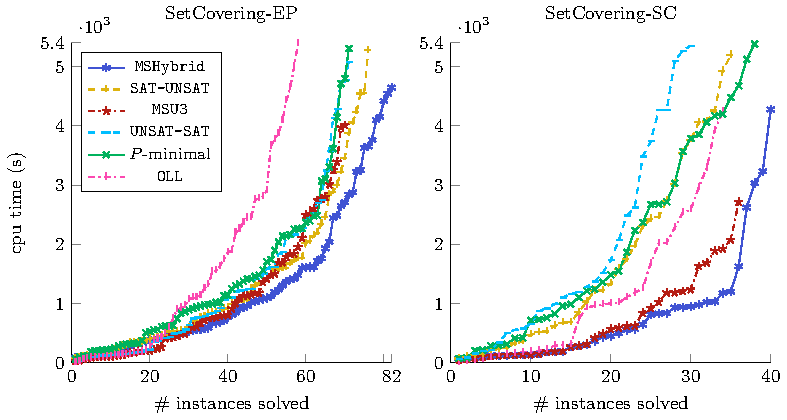
\includegraphics{setcover-cactus-single.pdf}
    \caption{Runtime comparison of $P$-minimal and variants of \algname{} for  bi-objective set covering problem.
      %The plot on the left is over instances generated with fixed probability that an element is in a set while the plot on the right is for instances with fixed set cardinality.
    }\label{fig:setcover-cactus}
\end{figure}

%Next, we compare \algname{} with $P$-minimal on  bi-objective set covering; see
%\Cref{fig:setcover-cactus} for a runtime comparison for
% fixed element probability instances (left) and fixed set cardinality instances (right).
% $P$-minimal  solves 71 (resp., 38) fixed element probability (resp., fixed set cardinality) instances,  while the best-performing \algname{} variant (\msh{}) solves
% 82 (resp., 40).

\begin{table}
  \centering
  \caption{Solved instances by approach and benchmark family.
%      The numbers are provided for computing a \emph{single} representative solution per pareto point or \emph{all} of them.
      %        The best approach per instance is highlighted in bold.
  }\label{tab:nsolved}
  \begin{tabular}{@{}lr@{\hskip 3pt}rr@{\hskip 3pt}rr@{\hskip 3pt}rr@{\hskip 3pt}rr@{\hskip 3pt}rr@{\hskip 3pt}r@{}}
    \toprule
    \multirow{2}{*}{Instance Type} & \multicolumn{2}{c}{\satunsat} & \multicolumn{2}{c}{\unsatsat} & \multicolumn{2}{c}{\msu} & \multicolumn{2}{c}{\oll} & \multicolumn{2}{c}{\msh} & \multicolumn{2}{c}{$P$-minimal} \\
    \cmidrule(r){2-3} \cmidrule(r){4-5} \cmidrule(r){6-7} \cmidrule(r){8-9} \cmidrule(r){10-11} \cmidrule(r){12-13}
    & single & all & single & all & single & all & single & all & single & all & {\hskip 6pt}single & all \\
    \midrule
    Decision Rules & 222 & \textbf{215} & 222 & \textbf{215} & 222 & \textbf{215} & 222 & 212 & \textbf{223} & \textbf{215} & 219 & 213 \\
    SetCovering-EP & 76 & 73 & 71 & 71 & 70 & 70 & 58 & 58 & \textbf{82} & \textbf{80} & 71 & 68 \\
    SetCovering-SC & 35 & 29 & 30 & 26 & 36 & 36 & 34 & 34 & \textbf{40} & \textbf{40} & 38 & 26 \\
    \bottomrule
  \end{tabular}
\end{table}

\begin{figure}
    \centering
    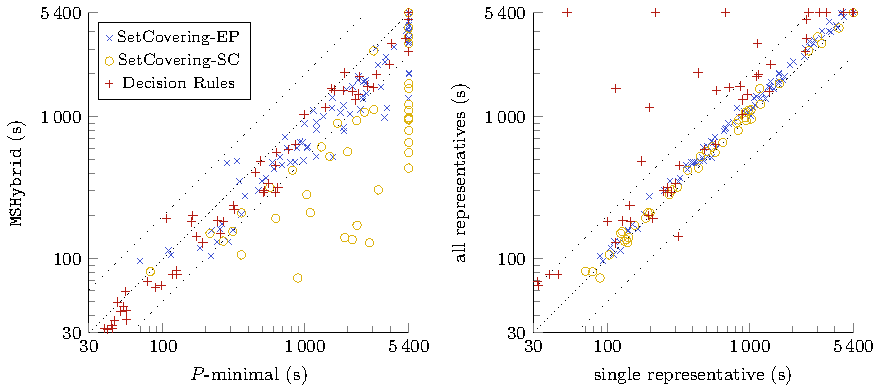
\includegraphics{all-datasets-combined-msh-and-enumeration.pdf}
    \caption{Left: Runtime comparison between $P$-minimal and \algname{} in the \msh{} variant. % over different instance types.
      Right: Runtime comparison between enumerating a single representative vs all solutions per pareto point with \msh{}.
%      point or all pareto-optimal solutions with the \msh{} variant.
      %        Instances with less than 30 seconds runtime are not shown.
    }\label{fig:msh-scatter}
\end{figure}

The numbers of solved instances are summarized in \cref{tab:nsolved},
both for  enumerating a single representative solution per pareto point and for enumerating \emph{all} pareto-optimal solutions.
\msh{} is the best-performing \algname{} variant overall, outperforming $P$-minimal in all cases. The performance difference
is greater when enumerating all pareto-optimal solutions.
For more details,
\cref{fig:msh-scatter} (left) shows a per-instance runtime comparison between \msh{} and $P$-minimal.
%In this plot, the dotted diagonal lines mark equal runtimes as well as double runtime in either direction.
We note that
$P$-minimal did not uniquely solve any instance. In general, \msh{} was outperformed by $P$-minimal on only 37 instances while \msh{} solves 308 instances in less time.
\Cref{fig:msh-scatter} (right) shows a runtime comparison between enumerating a single representative solution per pareto point and enumerating all pareto-optimal solutions with \msh{}.
 Overall, the approach scales well also for the latter task, although there understandably is an overhead 
  when the number of solutions required to be enumerated grows significantly; this is the case for
  LIDR
  where some instances
  have 
  more than $10,000$ solutions per pareto point.
This is in contrast to the set covering instances, which tend to have only a single (or few) solutions per pareto point.
%More details on enumerating all representative solutions with all approaches can be found in \cref{sup:plots}.
%  Since the set covering instances are weighted, and therefore it is significantly less likely that two solutions lead to the same objective values, these instances typically only have a single solution corresponding to every pareto point.
%Therefore, no significant difference in runtimes is visible for enumerating a single compared to all representative solutions.

\begin{figure}
    \centering
    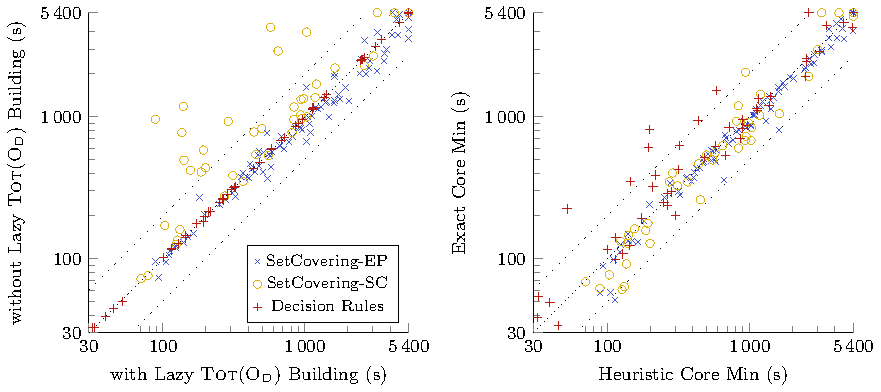
\includegraphics{all-datasets-chosen-refinements.pdf}
    \caption{Instance runtime comparisons for the two refinements lazily building the totalizer for the decreasing objective (left) and exact core minimization (right).
      %        Marker shapes and colours represent different instance types and instances with less than 30 seconds runtime are cropped out.}
      } \label{fig:refinements}
\end{figure}

Finally,
we evaluated the impact of the proposed refinements on the runtime efficiency of the best-performing approach, \msh{}.
%We consider two refinements in detail: lazily building $\tot(\Obj_\dec)$ and exact core minimization.
\Cref{fig:refinements} shows
the impact of lazily building $\tot(\Obj_\dec)$ (left) and exact vs heuristic core minimization (right).
Lazily building $\tot(\Obj_\dec)$ has no evident impact on LIDR,
as expected
(the literals from $\Obj_\dec$ do not appear in $\Obj_\inc$ and $\tot(\Obj_\dec)$ can therefore not be lazily built).
%For the set covering instances generated with fixed element probabilities, we see a slight negative effect for medium runtimes, but we have two instances that could only be solved when lazily building $\tot(\Obj_\dec)$.
For fixed set cardinality set covering, however, we see a strong positive effect.
%This is most likely due to the fact that the instances generated with fixed set cardinalities on average have more elements that don't appear in any of the sets and can therefore be left out of $\tot(\Obj_\dec)$.
Heuristic core minimization appears to have a positive effect  on LIDR as well as on harder set covering instances,
although the difference to exact minimization is smaller
than that of lazily building $\tot(\Obj_\dec)$.
%For set covering, exact core minimization has a slightly positive effect for instances that are solved in less time, for instances with long runtimes however, the effect is slightly negative.
%
%Other than those refinements, we also evaluated adding a
%The third refinement, i.e., disjoint phase to \msu{} which we found to have no lead to an improvement in performance.
%Data on this claim can be found in \cref{sup:plots}.